\documentclass{article}

\usepackage{amsmath, amssymb, algpseudocode, graphicx, amsthm}
\usepackage[margin=0.5in]{geometry}

\DeclareMathOperator*{\argmin}{arg\,min}
\DeclareMathOperator*{\argmax}{arg\,max}

\begin{document}

\title{Reinforcement Learning}
\author{Piyush Patil}
\maketitle

Reinforcement learning is an extremely general framework for the unsupervised trial-and-error style learning of arbitrary tasks, inspired by the positive and negative reinforcement feedback loops that govern how mammals learn. Recently, the intersection of deep neural networks and reinforcement learning methods has enabled very powerful machine learning systems. We begin our discussion with a review of the necessary background.

\section{Background}
The required background to fully explore the state-of-the-art in deep reinforcement learning requires an overview of modern deep learning methods as well as the fundamentals of reinforcement learning.

\subsection{Deep Learning}
The term deep learning was coined in contrast to conventional machine learning methods, such as SVMs, decision trees, linear and logistic regression, etc., which learning in a "shallow" way, in the sense that input vectors typically undergo a single mathematical transformation into an output vector, often with the application of manual feature engineering to the input vectors to increase the efficacy of the transformation. For example, linear and logistic regression both transform their inputs in such a way as to learn a linear or probabilistic model, and SVMs transform the input space so as to find a separating hyperplane. Deep learning, on the other hand, puts the input space through multiple layers of mathematical transformations, in an effort to hierarchically learn its own feature representations, layer by layer, so as to better augment the underlying model. Deep learning is thus characterized by its use of \textit{deep representations} of data, which are transformations built by composing many parameterized functions in a sequential chain; if every function in the composition is differentiable, we can use the chain rule to backpropagate error signals to each function's parameters.
\newline \newline
In the neural network approach, each layer takes the weighted sum of the components of its input vector, and passes through a non-linear activation function. In this way, the data flows forward, layer by layer, to produce an output. In supervised learning settings, we can compute an error signal by taking the derivative of a loss function with respect to our model parameters, ie the layer weights, and propagate the error signal backwards through the layers, nudging each parameter in a direction so as to lower the loss the next time around, until a local minimum of the loss function is reached. Deep neural networks have many layers; the idea is for later layers to learn high-level features in the data using lower-level features learned in previous layers. Each layer transforms the input into a feature vector that encodes features that the next layer can use to identify even higher-level features. Because the models we use tend to be end-to-end differentiable, manual feature engineering is unnecessary, since the entire model can be trained by backpropagating error signals, getting the model to learn its own feature representations.

\subsection{Reinforcement Learning}
Reinforcement learning is an extremely general framework designed for sequential decision making, and its definition is structured so as to mirror a general input-output feedback loop.
\newline \newline
\textbf{(Definition) Reinforcement learning}: \textit{Our model, which we will try to optimize through learning, is formulated as an \textbf{agent} that's situated in some \textbf{environment}, which it interacts with by taking an \textbf{action} and consequently receiving an \textbf{observation} as well as some interpretative \textbf{reward}. The model consists of an action-observation loop that proceeds in discrete time steps, so that at any given time $ t $ the model is determined by its history}
    $$ \left( (s_1, a_1, (o_1, r_1)), \cdots, (s_t, a_t, (o_t, r_t)) \right) $$
\indent \textit{where $ s_t $ is the current state, $ a_t $ is the action taken in state $ s_t $, and the agent makes an observation $ o_t $, revealing information about the environment, which includes a reward $ r_t $.}

\begin{center}
    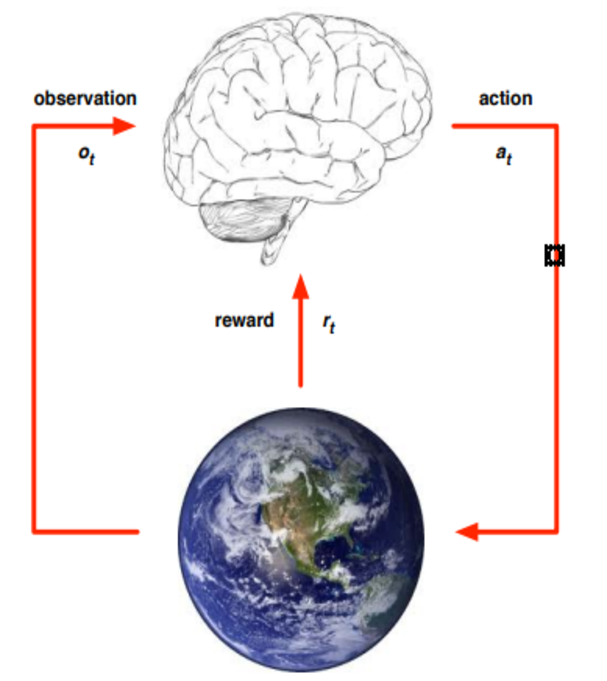
\includegraphics[scale=0.3]{images/rl_diagram.png}
\end{center}

At each time step, the agent sends an action to the environment and receives an observation and reward, while the environment sends an observation-reward pair to the agent, and receives an action.
\newline \newline
The environment of the reinforcement learning model is typically formulated as a \textbf{Markov decision process}. We can use that idea to formally define the full reinforcement learning setup.
\newline \newline
\textbf{(Definition) Markov decision process}: \textit{A \textbf{Markov decision process}, or MDP, is a tuple $ (\mathcal{S}, \mathcal{A}, T, R, \gamma) $ defined as follows.}
\begin{enumerate}
    \item \textit{A \textbf{state space} $ \mathcal{S} $, which is a set of states that fully determines the environment. At any given point, the agent is in some state.}
    \item \textit{An \textbf{action set} $ \mathcal{A} $, which is a full set of actions an agent can take. The agent interacts with subsets $ \mathcal{A}_s \subseteq \mathcal{A} $ of action sets, depending on the state $ s $.}
    \item \textit{A \textbf{state transition function} $ T: \mathcal{S} \times \mathcal{A} \rightarrow \mathcal{S} $, which is a mapping that determines the state at the next time step. It may or may not account for previous states (often just the last state), and may or may not be known to the agent. The function is usually modeled to be probabilistic, so that for every pair of states $ (s, s') $ and action $ a $,}
        $$ T(s, a) = s' \textit{ with probability } \Pr(s_{t + 1} = s' | (s_t, a_t) = (s, a)) $$
    \textit{Denote the induced probability distribution $ \mathcal{P} $.}
    \item \textit{A \textbf{reward function} $ R: \mathcal{S} \times \mathcal{A} \times \mathcal{S} \rightarrow \mathbb{R} $, which gives the agent a reward based what action it took from which state, and what the next state was as a result. Thus,}
        $$ R(s_t, a_t, s_{t + 1}) = \textit{ reward for taking action $ a_t $ to transition from state $ s_t $ to $ s_{t + 1} $ } $$
    \item \textit{A \textbf{discount factor} $ \gamma \in [0, 1] $, which is the ratio between how much the value of a reward is worth in the next time step relative to the current time step, the idea being that our agent should value sooner rewards more than later ones.}
\end{enumerate}
%\newline \newline
Notice that the determination of what the next state is depends only on the current state and the action take in the current state, and not on the entire history of states and actions up to that point. Thus, MDPs have the Markov property that defines Markov chains, to which they owe their names; in practice, systems don't always follow the Markov property and hence the state space definition must be modified so as to force the current state to encode all the relevant information about the history. The goal in reinforcement learning is to find a \textbf{policy} for choosing actions in states. More formally, we want to learn a policy function $ \pi: \mathcal{S} \rightarrow \mathcal{A} $ which chooses which action to take, depending on the current state. In general, our policy may not be a deterministic function as above but rather might simply associate to each state a probability distribution over the action space of that state, in which case we have a stochastic policy. The search for a policy is why we incorporate the notion of a reward into the requirement; depending on what the goal of the overall task is, different observations from the environment may be positive or negative. We want to choose a policy that's best aligned with the goal, in the sense that it maximizes the expected total discounted reward we receive from the environment, ie we want to maximize the "value" of a state, formalized below.
\newline \newline
\textbf{(Definition) Value function}: \textit{The \textbf{value function} for a policy $ \pi: \mathcal{S} \rightarrow \mathcal{A} $ is the function $ V^\pi: \mathcal{S} \rightarrow \mathbb{R} $ given by}
    $$ V^\pi(s) := \underset{s' \sim \mathcal{P} | (s, \pi(s))}{\mathbb{E}} \left[ \sum_{t = 0}^\infty \gamma^t R(s, \pi(s), s') \right] $$
\textit{where the expectation is over the probability distribution of the state transition function.}
\newline \newline
This function formalizes our best estimate for the value of a particular state $ s $, as the expected total discounted reward. It's often convenient to define a similar \textbf{action value function} to formally estimate the value of taking an action from a state:
    $$ Q(s, a) = \underset{s' \sim \mathcal{P} | (s, a)}{\mathbb{E}} \left[ \sum_{t = 0}^\infty \gamma^t R(s, a, s') \right] $$
so that $ V^\pi(s) = Q(s, \pi(s)) $. It follows that we can instead recursively define the state value function for policy $ \pi $ at time step $ t $ as
    $$ V^\pi(s) = r(s) + \gamma \sum_{s' \in \mathcal{S}} \Pr(s' | (s, \pi(s))) V^\pi(s') \text{ where } r(s) = \underset{s' \sim \mathcal{P} | (s, \pi(s))}{\mathbb{E}} \left[ R(s, \pi(s), s') \right] = \sum_{s' \in \mathcal{S}} \Pr(s' | (s, \pi(s))) R(s, \pi(s), s') $$
where $ r(s) $ is the expected reward received for entering state $ s $, taken over all possible previous state-action combinations. This is known as the \textbf{Bellman equation}. For finite MDPs, in which $ \mathcal{S} $ is finite, we can simply write $ | \mathcal{S} | $ Bellman equations as above, one for each $ s \in \mathcal{S} $, giving us a system of linear equations in $ | \mathcal{S} | $ equations and $ | \mathcal{S} | $ unknowns, namely the $ V^\pi(s) $'s, for each $ s \in \mathcal{S} $. By solving the system, we can find an explicit description of $ V^\pi $.
\newline \newline
Usually we're interested in a higher goal, however. Rather than computing the value function, our overall goal is to find a policy $ \pi $ that maximizes the value function. Define the \textbf{optimal value function} as follows.
    $$ V^*(s) = \max_\pi V^\pi(s) = r_t + \max_{a \in \mathcal{A}} \gamma \sum_{s' \in \mathcal{S}} \Pr(s' | (s, a)) V^*(s') $$
The corresponding optimal policy, then, is given by
    $$ \pi^*(s) = \argmax_{a \in \mathcal{A}} \sum_{s' \in \mathcal{S}} \Pr(s' | (s, a)) V^*(s') $$
From the way we've defined $ V^* = V^{\pi^*} $, it's necessarily true that for every state $ s $ and policy $ \pi $, $ V^*(s) \geq V^\pi(s) $. This aligns with the subtle assumption we've made here that the optimal policy is a deterministic lookup table mapping states to actions, and so we can always use $ \pi^* $ as our policy no matter what the MDP is.

\section{Conventional Reinforcement Learning}
The three major components of a reinforcement learning agent are its policy, which governs how it acts, its value function, which governs how it rates states and actions, and its model, which is it's representation of the environment (typically, the exact transition and reward functions are not known or are not computable). RL techniques can try to optimize and learn any combination of these three components. Thus, in general the field of RL breaks down into value-based RL, wherein we estimate the optimal value function (which can be either $ V^* $ or $ Q^* $), policy-based RL, where we search directly for an optimal policy, and model-based RL, where we build a strong model of the environment with as much information as possible, use the model to implement strategic planning-based learning that looks ahead in future time steps based on the model. In practice, when using reinforcement learning in real-world applications, building a good model and adapting it to the standard RL/MDP setup we've laid out can be a major bottleneck. The world tends to be very large and complex, and it's often the case that we only receive concrete reward signals at the end of long sequences of actions (such as board games, when the win or loss is only discovered at the end), making it difficult to determine which actions were responsible for the reward. This is known as the \textit{credit assignment problem}. Although in theory this doesn't affect the optimality of the learning algorithms we discuss below, in practice it can make converence intractably slow or unstable. Let's start by looking at some simple ways of solving finite MDPs.

\subsection{Value and Policy Iteration}
There are two primary efficient algorithms for solving finite MDPs, which we assume have finite state and action spaces. The first algorithm is called \textbf{value iteration}. The basic idea behind value iteration is to simply use the Bellman equation for the optimal value function to start with a null (or random) value function and iteratively update it, in the hope that it will eventually be forced to follow the Bellman equation and hence converge to $ V^* $. Thus, the algorithm is

\begin{algorithmic}
    \Procedure{ValueIteration}{}
        \State Initialize $ \forall s \in \mathcal{S}: V(s) \gets 0 $
        \While{$ V $ has not converged}
            \For{$ s \in \mathcal{S} $}
                \For{$ a \in \mathcal{A} $}
                    \State $ Q(s, a) \gets \underset{s' \sim \mathcal{P} | (s, a)}{\mathbb{E}} [ R(s, a, s') + \gamma V(s') ] = r(s) + \gamma \sum \limits_{s' \in \mathcal{S}} \Pr(s' | (s, a)) V(s') $
                \EndFor
                \State $ V(s) \gets \max \limits_{a \in \mathcal{A}} Q(s, a) $
            \EndFor
        \EndWhile
    \EndProcedure
\end{algorithmic}

This simple greedy algorithm, it turns out, can be proven to converge to the optimal value function, which we can then use to compute the optimal policy. Policy iteration, on the other hand, directly searches for the optimal policy, also by using the Bellman equation, but skipping over any explicit learning of the value function.

\begin{algorithmic}
    \Procedure{PolicyIteration}{}
        \State Initialize $ \pi $ randomly
        \While{$ \pi $ has not converged}
            \State $ V \gets V^\pi $
            \For{$ s \in \mathcal{S} $}
                \State $ \pi(s) \gets \argmax \limits_{a \in \mathcal{A}} \sum \limits_{s' \in \mathcal{S}} \Pr(s' | (s, a)) V(s') $
            \EndFor
        \EndWhile
    \EndProcedure
\end{algorithmic}

In both algorithms above, $ \Pr(s' | (s, a)) = T(s, a, s') $. The step $ V = V^\pi $ involves computing the value function, possibly by solving the system of $ | \mathcal{S} | $ linear equations above. The algorithm essentially computes the value function for the current policy, then updates by re-selecting $ \pi $'s state-action mapping depending on the value function. Both value and policy iteration are guaranteed to converge to the optimal policy in finite time.
\newline \newline
Before wrapping up the section, let's formally prove this statement, phrased mathematically as follows.
\newline \newline
\textbf{(Theorem) Convergence of Value Iteration}: \textit{Define the \textbf{Bellman backup operator} $ T: \mathbb{R}^\mathcal{S} \rightarrow \mathbb{R}^\mathcal{S} $ on the subspace of value functions as defined above with}
    $$ \forall \textit{ value functions } V: \forall s \in \mathcal{S}: T[V](s) = \max_{a \in \mathcal{A}} \left( r(s, a) + \gamma \sum_{s' \in \mathcal{S}} \Pr(s' | (s, a)) V(s') \right) $$
\textit{Then, denoting the optimal value function with $ V^* $, we have}
    $$ \forall V \in \mathbb{R}^\mathcal{S}: \lim_{H \to \infty} T^H[V] = \lim_{H \to \infty} \overbrace{T[T[\cdots T[V]]]}^\text{$ H $ times} = V^* $$
\indent \textit{Proof}: For some fixed horizon $ H $, we can write the value function corresponding to policy $ \pi $ as
    $$ V^\pi(s) = \mathbb{E} \left[ \sum_{t = 0}^\infty \gamma^t R(s_t) \right] = \mathbb{E} \left[ \sum_{t = 0}^{H - 1} \gamma^t R(s_t) \right] + \mathbb{E} \left[ \sum_{t = H}^\infty \gamma^t R(s_t) \right] $$
where the expectation is over the probability distribution induced by the underlying MDP's transition function, conditioned on the state-action pair $ (s, \pi(s)) $, defining the next state $ s' $, and $ R(s_t) $ is the expected reward from state $ s_t $ at time $ t $ if we follow $ \pi $ for $ t $ time steps. Recall that the $ L_\infty $-norm of a function is, by definition, an upper bound on that function. Thus, assuming our value function and hence the reward function is bounded, we have
    $$ \mathbb{E} \left[ \sum_{t = H}^\infty \gamma^t R(s_t) \right] \leq \sum_{t = H}^\infty \gamma^t || R ||_\infty = \frac{\gamma^H}{1 - \gamma} || R ||_\infty $$
We can use this geometric bound to find lower and upper bounds on $ T^H[V] $, which will, in the limit, squeeze the operator to the optimal policy. First, intuitively we'd expect that
    $$ \forall s \in \mathcal{S}: T^H[V](s) = \max_\pi \mathbb{E} \left[ \sum_{t = 0}^{H - 1} \gamma^t R(s_t) + \gamma^H V(s) \right] $$
since we want $ T[V] $ to iteratively optimize $ V $, and since the operator is defined as the maximum reward over the action space. We can prove this by induction, since
    $$ \begin{aligned}
        \forall s \in \mathcal{S}: T^{H + 1}[V](s) &= \max_{a \in \mathcal{A}} \left( r(s, a) + \gamma \sum_{s' \in \mathcal{S}} \Pr(s' | (s, a)) T^H[V](s') \right) \\
        &= \max_{a \in \mathcal{A}} \left( r(s, a) + \gamma \sum_{s' \in \mathcal{S}} \Pr(s' | (s, a)) \max_\pi \mathbb{E} \left[ \sum_{t = 0}^{H - 1} \gamma^t R(s_t) + \gamma^H V(s') \right] \right) \text{ where } s_H = s \\
        &= \max_\pi \left( r(s, \pi(s)) + \gamma \sum_{s' \in \mathcal{S}} \Pr(s' | (s, a)) \mathbb{E} \left[ \sum_{t = 0}^{H - 1} \gamma^t R(s_t) \right] + \gamma \sum_{s' \in \mathcal{S}} \Pr(s' | (s, \pi(s))) \gamma^H V(s') \right) \\
        &= \max_\pi \left( \mathbb{E} \left[ \sum_{t = 0}^H \gamma^t R(s_t) \right] + \gamma^{H + 1} V(s))) \right) \\
        &= \max_\pi \mathbb{E} \left[ \sum_{t = 0}^H \gamma^t R(s_t) + \gamma^{H + 1} V(s) \right]
    \end{aligned} $$
where $ r(s, a) $ is the expected reward from taking action $ a $ in state $ s $. We can ignore the maximum over the action space since the maximum over all policies implies taking the optimal action. It follows that
    $$ \begin{aligned}
        \forall s \in \mathcal{S}: T^H[V](s) &= \max_\pi \mathbb{E} \left[ \sum_{t = 0}^{H - 1} \gamma^t R(s_t) + \gamma^H V(s) \right] \\
        &\leq \max_\pi \mathbb{E} \left[ \sum_{t = 0}^{H - 1} \gamma^t R(s_t) + \sum_{t = H}^\infty \gamma^t R(s_t) + \gamma^H V(s) + \frac{\gamma^H}{1 - \gamma} || R ||_\infty  \right] \text{ since } \sum_{t = H}^\infty \gamma^t R(s_t) + \frac{\gamma^H}{1 - \gamma} || R ||_\infty \geq 0 \\
        &= \max_\pi \mathbb{E} \left[ \sum_{t = 0}^\infty \gamma^t R(s_t) \right] + \gamma^H \max_\pi \mathbb{E}[V(s)] + \frac{\gamma^H}{1 - \gamma} || R ||_\infty \\
        &\leq V^*(s) + \gamma^H || V ||_\infty + \frac{\gamma^H}{1 - \gamma} || R ||_\infty
    \end{aligned} $$
Symmetrically,
    $$ \begin{aligned}
        \forall s \in \mathcal{S}: T^H[V](s) &= \max_\pi \mathbb{E} \left[ \sum_{t = 0}^{H - 1} \gamma^t R(s_t) + \gamma^H V(s) \right] \\
        &\geq \max_\pi \mathbb{E} \left[ \sum_{t = 0}^{H - 1} \gamma^t R(s_t) + \sum_{t = H}^\infty \gamma^t R(s_t) + \gamma^H V(s) - \frac{\gamma^H}{1 - \gamma} || R ||_\infty  \right] \text{ since } \sum_{t = H}^\infty \gamma^t R(s_t) + \frac{\gamma^H}{1 - \gamma} || R ||_\infty \geq 0 \\
        &= \max_\pi \mathbb{E} \left[ \sum_{t = 0}^\infty \gamma^t R(s_t) \right] + \gamma^H \max_\pi \mathbb{E}[V(s)] - \frac{\gamma^H}{1 - \gamma} || R ||_\infty \\
        &\geq \max_\pi \mathbb{E} \left[ \sum_{t = 0}^\infty \gamma^t R(s_t) \right] - \gamma^H \max_\pi \mathbb{E}[V(s)] - \frac{\gamma^H}{1 - \gamma} || R ||_\infty \\
        &\geq V^*(s) - \gamma^H || V ||_\infty - \frac{\gamma^H}{1 - \gamma} || R ||_\infty
    \end{aligned} $$
It follows that
    $$ \forall s \in \mathcal{S}: \lim_{H \to \infty} \left( V^*(s) - \gamma^H || V ||_\infty - \frac{\gamma^H}{1 - \gamma} || R ||_\infty \right) \leq \lim_{H \to \infty} T^H[V](s) \leq \lim_{H \to \infty} \left( V^*(s) - \gamma^H || V ||_\infty + \frac{\gamma^H}{1 + \gamma} || R ||_\infty \right) $$
    $$ \rightarrow \forall s \in \mathcal{S}: V^*(s) - \left( || V ||_\infty + \frac{1}{1 - \gamma} || R ||_\infty \right) \lim_{H \to \infty} \gamma^H \leq \lim_{H \to \infty} T^H[V](s) \leq V^*(s) + \left( || V ||_\infty + \frac{1}{1 - \gamma} \right) \lim_{H \to \infty} \gamma^H $$
    $$ \rightarrow \forall s \in \mathcal{S}: \lim_{H \to \infty} T^H[V](s) = V^*(s) \text{ since } \lim_{H \to \infty} \gamma^H = 0 $$
and hence $ \lim \limits_{H \to \infty} T^H[V] = V^* $. \qedsymbol
\newline \newline
The convergence of policy iteration follows from the convergence of value iteration, since we defined our optimal policy function in terms of the definition of the optimal value function above.

\subsubsection{Learning the Model}
Both value and policy iteration require that the state transition and reward functions are both known ahead of time. In general reinforcement learning settings, this is often not the case; often, the environment is completely unknown. In such settings, we'd like to implement some mode of trial-and-error learning that allows the agent to gradually learn the state transition and reward functions over time, jointly with the optimal policy. This is a kind of \textit{active learning}, wherein the agent explores the search space and trying different actions in an attempt to find the best policy, as opposed to the \textit{passive learning} approach taken by value and policy iteration, in which the agent acts according to a fixed policy and tries to learn how good the policy is by observing the world.
\newline \newline
\textit{Direct utility estimation} is a simple, general way, inspired by Monte Carlo methods, to learn these functions over time through sampling. Specifically, after undergoing several iterations of the state-action-observation loop, we can approximate
    $$ \Pr(s' | (s, a)) \gets \frac{\text{number of times we transitioned $ (s, a) \mapsto s' $}}{\text{number of times we've taken action $ a $ from state $ s $}} $$
We can accumulate this probability over time as our history grows, eventually converging, by the central limit theorem, to the true transition probabilities, starting with an initial uniform distribution, where every state probability is $ | \mathcal{S} |^{-1} $. Similarly, we can continuously update
    $$ R(s, a, s') \gets \text{ average reward from the transition $ (s, a) \mapsto s' $ } $$
We can either perform each update once per iteration, learning them jointly with the policy or value function, or, in a more general version of trial-and-error, take some fixed number of random steps to "gather data" and update the state transition function and reward function approximations accordingly. The former case is similar to stochastic gradient descent and is faster but carries more noise, while the latter updates in "batches" that force the functions to converge faster, but require data collection periods where the policy or value function isn't updated at all. This approach has several drawbacks, such as only being valid for finite (and in practice, rather small) MDPs, and has a rate of convergence proportional to the variance of the value function, which might be high.
\newline \newline
\textit{Adaptive dynamic programming} is a method proposed to deal with some of the drawbacks of direct utility estimation, in particular its very slow rate of convergence, we modify the algorithm to make use of another source of information that it missed - the fact that at any given point the transition and reward functions must satisfy the Bellman equations. In this method, we learn the value function through sampling, computing a certain number of samples of the form
$$ \forall i \in \{ 1, \cdots, n \}: S_i \gets = R(s, \pi(s), s_i') + \gamma V^\pi(s) \text{ where } s_i' = \text{ future state } $$
allowing us to approximate the value function by averaging our samples:
$$ V^\pi(s) \gets V^\pi(s) + \frac{\alpha}{n} \sum_{i = 1}^n S_i $$
for learning rate $ \alpha $.

\subsection{Value-Based Methods}
Value-based methods try to find a good policy, which maximizes the infinite-horizon discounted reward (that is, the sum of all future discounted rewards), by computing the value function for a given policy that's iteratively updated over time, based on its value.

\subsubsection{Temporal Difference Learning}
TD learning is a middle ground between Monte Carlo sampling methods and dynamic programming methods to learn the value function. In both value and policy iteration, even when interspersed with model learning methods, we update our policy for a given state by computing an expectation over the entire state space. This expectation, of course, relies on our current estimate of the value function, and so we use the current estimate of the value function at each state in the state space to compute (our approximation to) this expectation, which is then used in our updates. This is strongly aligned with the standard supervised learning paradigm, wherein we run our model to completion and subsequently update by comparing to a label. A commonly used example is that if we wanted to predict the weather for a week, we'd formulate a model first, tabulate error signals for each day up until Saturday, and then update the model.
\newline \newline
However, this throws away information that could speed up convergence. As each day passes, we can backpropagate each error signal for that day and immediately update our model iteratively, so that by Saturday the model we use to predict the weather is much better than the one we started with. This is the central idea behind TD learning. Over an episode of $ T $ time steps in which we approximate the value function, rather than accumulating an update term after the $ T $ time steps that's based on an expectation computed over those time steps, we compute $ T - 1 $ updates, one after each time step, and immediately re-compute a slightly improved value function with each update. In a prediction task, rather than computing updates using the difference between actual and predicted outcomes, we compute updates using differences between temporally successive predictions. Let's now formally define the algorithm.
\newline \newline
Before looking at the full algorithm, we motivate it in a simpler context, before then applying it to our reinforcement learning framework. In the general \textit{infinite-horizon discounted prediction problem} setup, we receive as input $ (o_t, r_t) \in X \times \mathbb{R}^+ $ at each time step $ t $. The $ o_t $ are observations drawn from some vector space $ X $, usually simply $ n $-dimensional Euclidean space, and the $ r_t $ are positive reward signals. We seek a function $ f: X \rightarrow \mathbb{R}^+ $ for predicting, at time $ t $, the value
    $$ R_t = r_{t + 1} + \gamma r_{t + 2} + \gamma^2 r_{t + 3} + \cdots = \sum_{i = 0}^\infty \gamma^i r_{t + i + 1} $$
We'll define a sequence of functions $ ( f_t ) $ that we'll construct by updating $ f_{t - 1} $ to produce $ f_t $, with the hope of converging towards a minimal value of some loss function between $ f_t(\cdot) $ and $ R_t $. Suppose further for the sake of simplicity that $ X $ is finite, so that updating our prediction function $ f $ can be done by updating entries in a lookup table (we'll generalize this to continuous domains later). In the case where $ \gamma = 0 $, and we simply want to predict $ r_{t + 1} $ given $ o_t $ and don't care about future values, we can implement an update rule by directly propagating the error in our prediction to our prediction function:
    $$ f_{t + 1}(o_t) \gets f_t(o_t) + \alpha \cdot (r_{t + 1} - f_t(o_t)) $$
where $ \alpha \in [0, 1] $ is a learning rate. When $ \gamma > 0 $, however, we would have to wait an infinite number of time steps to receive our error signal and propagate it. We can avoid this with a simple approximation - notice that
    $$ R_t = \sum_{i = 0}^\infty \gamma^i r_{t + i + 1} = r_{t + 1} + \gamma \sum_{i = 1}^\infty \gamma^{i - 1} r_{t + i + 1} = r_{t + 1} + \gamma \sum_{i = 0}^\infty \gamma^i r_{(t + 1) + i + 1} = r_{t + 1} + \gamma R_{t + 1} $$
and we can approximate $ R_{t + 1} $ by using our current prediction, ie with $ f_t(o_{t + 1}) $. Then, if we define our \textit{temporal difference error} to be
    $$ \delta_{t + 1} = r_{t + 1} + \gamma f_t(o_{t + 1}) - f_t(o_t) $$
we have the update
    $$ f_{t + 1}(o) = \begin{cases}
        f_t(o) + \alpha \delta_{t + 1}, &\text{ if } o = o_t \\
        f_t(o), &\text{ otherwise }
    \end{cases} $$
In continuous domains, when $ X $ is not finite, we can parameterize our function $ f_t $ with some $ \theta $ over some parameter space. Let $ ( f_t^\theta ) $ denote the function space over this parameter space. Given some loss function $ L $ we can update with gradient descent over $ \theta $. If $ \theta_t $ is our parameterization at time $ t $, then upon receiving our observation and reward pair, we update
    $$ \theta_{t + 1} \gets \theta_t + \alpha \delta_{t + 1} \nabla_{\theta_t} L $$
In our reinforcement learning setting, this means that our Monte Carlo update equation above, in which we sampled $ n $ times and updated our estimate of the value function with the average of the $ n $ samples, now becomes
    $$ V^\pi(s) \gets V^\pi(s) + \alpha \cdot (S - V^\pi(s)) \text{ where } S = R(s, \pi(s), s') + \gamma V^\pi(s) \text{ for future state } s' $$
This idea of learning from both observation and our own model's predictions so far is known as \textit{bootstrapping}, and speeds up convergence in general prediction problems.

\subsubsection{$ Q $-learning}
Recall that instead of a state value function $ V^\pi $ we can define a state-action function $ Q $ so that $ V^\pi(s) = Q(s, \pi(s)) $. The objective of $ Q $-learning is to learn the optimal state-action function
    $$ Q^*(s, a) := r(s, a) + \gamma \sum_{s' \in \mathcal{S}} \Pr(s' | (s, a)) \max_{a' \in \mathcal{A}} Q^*(s', a') \text{ where } r(s, a) = \underset{s' \sim \mathcal{P} | (s, a)}{\mathbb{E}} \left[ R(s, a, s') \right] = \sum_{s' \in \mathcal{S}} \Pr(s' | (s, a)) R(s, a, s') $$
where $ r(s, a) $ is the expected reward from taking action $ a $ in state $ s $. This is equivalent to learning the value function instead, since we have
    $$ V^*(s) = \max_{a \in \mathcal{A}} Q^*(s, a) \text{ and } \pi^*(s) = \argmax_{a \in \mathcal{A}} Q^*(s, a) $$
In contrast to value iteration, which learns the value function and is generally used when the transition probabilities and possible state transitions are known, $ Q $-learning is completely model-free, and is often more computationally tractable (since it starts with no knowledge of the state) than repeatedly enumerating very large state spaces. The update rule is very similar to that in temporal difference learning with value iteration:
    $$ \forall s \in \mathcal{S}, a \in \mathcal{A}: Q_{t + 1}(s, a) \gets Q_t(s, a) + \alpha \cdot (r_{t + 1} + \gamma \max_{a' \in \mathcal{A}} Q(s', a') - Q(s, a)) $$
where $ s' $ is the state we dropped into after taking action $ a $ from action $ a $, and $ r_{t + 1} $ is the received reward. Note that the update is performed after the action has been executed, and $ s' $ and $ r_{t + 1} $ have been revealed to the agent. Like value iteration, these updates are guaranteed to converge to $ Q^* $ in finite time.

\subsection{Policy-Based Methods}
Other ways of finding a good policy is to directly search for one under some formulation. \textit{Gradient-based methods} do this by parameterizing some space of possible policy functions and hill climbing towards an optimal policy. Specifically, given a parameter vector $ \theta $ we have a class of possible policies $ \{ \pi_\theta, \theta \in X \} $ for some finite-dimensional vector space of parameters $ X $. In many cases, we can impose mild conditions on the policy function so as to allow the performance function 
    $$ \rho(\theta) = \text{ performance of } \pi^\theta \text{ with respect to discounted reward } $$
to be computable and differentiable (the above definition of a performance function is very general, and in practice there are many different implementations of a performance function over a space of policies). Though it's often difficult to analytically compute the gradient of $ \rho $, we can simply use gradient ascent to find a good policy. Of course, an immediate drawback to this approach is getting stuck in local minima. Moreover, because gradient ascent relies on individual samples of the gradient, which inevitably will be noisy and hence only be a faithful representation of the gradient in expectation, convergence might be very slow depending on the amount of noise. There do exist \textit{gradient-free} methods for optimizing $ \rho $, such as simulated annealing, evolutionary algorithms, or some cross-entropy methods, which can, in theory and sometimes in practice, find global optima.

\subsubsection{SARSA}
TODO

\subsubsection{REINFORCE}

\subsection{Actor-Critic Methods}

\subsubsection{Asynchronous Advantage Actor-Critic}
A3C

\section{Deep Reinforcement Learning}
Deep reinforcement learning refers to any RL method wherein deep neural networks are used to approximate some component of the MDP setup, such as the value function, the $ Q $ function, the policy, or the environment. The model can then be trained with gradient descent methods.

\subsection{Deep $ Q $-Networks}
https://storage.googleapis.com/deepmind-data/assets/papers/DeepMindNature14236Paper.pdf

\subsubsection{Prioritised Replay}

\subsubsection{Duelling Network}

\subsubsection{Double $ Q $-Learning}

\subsection{Policy Optimization}

\subsubsection{Deterministic Policy Gradients}
https://arxiv.org/pdf/1509.02971.pdf

\subsubsection{Guided Policy Search}

\section{Inverse Reinforcement Learning}

\subsection{Apprenticeship Learning}

\section{Planning}

\subsection{Value Iteration Networks}
https://arxiv.org/pdf/1602.02867.pdf

\end{document}
